\documentclass[aspectratio=43]{beamer}

% Text packages to stop warnings
\usepackage{lmodern}
\usepackage{textcomp}
\usepackage[utf8]{inputenc}
\usepackage[T1]{fontenc}
\usepackage{ulem}
\usepackage{listings}
%% \usetikzlibrary{arrows,automata,shapes}
%% \tikzstyle{block} = [rectangle, draw, fill=blue!20, 
%%     text width=2.5em, text centered, rounded corners, minimum height=2em]
%% \tikzstyle{bw} = [rectangle, draw, fill=blue!20, 
%%     text width=3.5em, text centered, rounded corners, minimum height=2em]

% Themes
\usetheme{Boadilla}
\setbeamertemplate{footline}[page number]{}
\setbeamertemplate{navigation symbols}{}
\newtheorem{defn}{Definition}

% Suppress the navigation bar
\beamertemplatenavigationsymbolsempty

\newenvironment{changemargin}[1]{% 
  \begin{list}{}{% 
    \setlength{\topsep}{0pt}% 
    \setlength{\leftmargin}{#1}% 
    \setlength{\rightmargin}{1em}
    \setlength{\listparindent}{\parindent}% 
    \setlength{\itemindent}{\parindent}% 
    \setlength{\parsep}{\parskip}% 
  }% 
  \item[]}{\end{list}} 

\lstset{basicstyle=\scriptsize, frame=single}

\title{Lecture 34---Password cracking on GPUs; reduced-resource computation; STM}
\subtitle{ECE 459: Programming for Performance}
\date{March 30, 2015}

\lstdefinelanguage{scala}{
  morekeywords={abstract,case,catch,class,def,%
    do,else,extends,false,final,finally,%
    for,if,implicit,import,match,mixin,%
    new,null,object,override,package,%
    private,protected,requires,return,sealed,%
    super,this,throw,trait,true,try,%
    type,val,var,while,with,yield},
  otherkeywords={=>,<-,<\%,<:,>:,\#,@},
  sensitive=true,
  morecomment=[l]{//},
  morecomment=[n]{/*}{*/},
  morestring=[b]",
  morestring=[b]',
  morestring=[b]"""
}


\begin{document}
%%%%%%%%%%%%%%%%%%%%%%%%%%%%%%%%%%%%%%%%%%%%%%%%%%%%%%%%%%%%%%%%%%%%%%%%%%%%%%%%
\begin{frame}[plain]
  \titlepage
\end{frame}
%%%%%%%%%%%%%%%%%%%%%%%%%%%%%%%%%%%%%%%%%%%%%%%%%%%%%%%%%%%%%%%%%%%%%%%%%%%%%%%%

%%%%%%%%%%%%%%%%%%%%%%%%%%%%%%%%%%%%%%%%%%%%%%%%%%%%%%%%%%%%%%%%%%%%%%%%%%%%%%%%
\begin{frame}
  \frametitle{Last Time: OpenCL}

  Saw principles of OpenCL programming:

  \begin{center}
    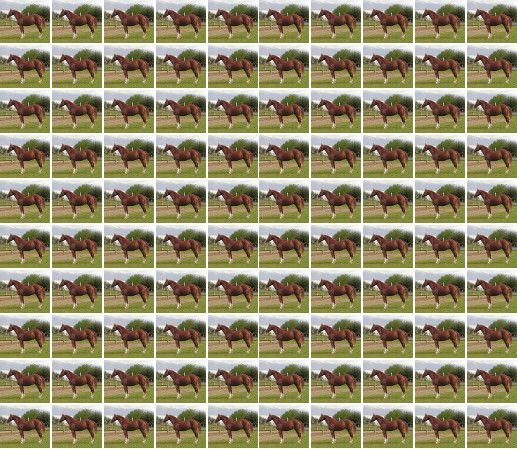
\includegraphics[width=.6\textwidth]{L34/100-horses.jpg}
  \end{center}
  \hfill {\small (Credit: Karlyne, Wikimedia Commons)}
  % http://en.wikipedia.org/wiki/File:Avenger_-_Westphalian_horse.jpg

  Key concepts: kernels, buffers.
  
\end{frame}
%%%%%%%%%%%%%%%%%%%%%%%%%%%%%%%%%%%%%%%%%%%%%%%%%%%%%%%%%%%%%%%%%%%%%%%%%%%%%%%%

\part{GPU Application: Password Cracking}
\frame{\partpage}

%%%%%%%%%%%%%%%%%%%%%%%%%%%%%%%%%%%%%%%%%%%%%%%%%%%%%%%%%%%%%%%%%%%%%%%%%%%%%%%%
\begin{frame}
  \frametitle{Reference: scrypt}

  \begin{changemargin}{2cm}
    scrypt is the algorithm behind DogeCoin. \\[1em] The reference:\\[1em]
    
    Colin Percival, ``Stronger Key Derivation via Sequential Memory-Hard Functions''. \\
    Presented at BSDCan'09, May~2009.\\[1em]

    \url{http://www.tarsnap.com/scrypt.html}
  \end{changemargin}
\end{frame}
%%%%%%%%%%%%%%%%%%%%%%%%%%%%%%%%%%%%%%%%%%%%%%%%%%%%%%%%%%%%%%%%%%%%%%%%%%%%%%%%

%%%%%%%%%%%%%%%%%%%%%%%%%%%%%%%%%%%%%%%%%%%%%%%%%%%%%%%%%%%%%%%%%%%%%%%%%%%%%%%%
\begin{frame}
  \frametitle{Acceptable Practices for Password Storage}
  \begin{changemargin}{2cm}
    \begin{itemize}
    \item {\Huge \alert{{\bf not} plaintext!}}
    \item \Large hashed and salted
    \end{itemize}
       
\end{changemargin}
\end{frame}
%%%%%%%%%%%%%%%%%%%%%%%%%%%%%%%%%%%%%%%%%%%%%%%%%%%%%%%%%%%%%%%%%%%%%%%%%%%%%%%%

%%%%%%%%%%%%%%%%%%%%%%%%%%%%%%%%%%%%%%%%%%%%%%%%%%%%%%%%%%%%%%%%%%%%%%%%%%%%%%%%
\begin{frame}
  \frametitle{Cryptographic hashing}
  \begin{changemargin}{2cm}
    One-way function:
    \begin{itemize}
    \item $x \mapsto f(x)$ ~~easy to compute; but
      \item $f(x) \stackrel{?~}{\mapsto} x$ ~~hard to reverse.
    \end{itemize}~\\
    Examples: SHA1, Scrypt.
\end{changemargin}
\end{frame}
%%%%%%%%%%%%%%%%%%%%%%%%%%%%%%%%%%%%%%%%%%%%%%%%%%%%%%%%%%%%%%%%%%%%%%%%%%%%%%%%

%%%%%%%%%%%%%%%%%%%%%%%%%%%%%%%%%%%%%%%%%%%%%%%%%%%%%%%%%%%%%%%%%%%%%%%%%%%%%%%%
\begin{frame}
  \frametitle{Breaking the Hash}
  \begin{changemargin}{2cm}
    How can we reverse the hash function?
    \begin{itemize}
    \item    Brute force.
    \end{itemize}~\\
    GPUs (or custom hardware) are good at that!
  \end{changemargin}
\end{frame}
%%%%%%%%%%%%%%%%%%%%%%%%%%%%%%%%%%%%%%%%%%%%%%%%%%%%%%%%%%%%%%%%%%%%%%%%%%%%%%%%

%%%%%%%%%%%%%%%%%%%%%%%%%%%%%%%%%%%%%%%%%%%%%%%%%%%%%%%%%%%%%%%%%%%%%%%%%%%%%%%%
\begin{frame}
  \frametitle{The Arms Race: Making Cracking Difficult}
  \begin{changemargin}{2cm}
    Historically: force repeated iterations of hashing.\\[1em]

    Main idea behind scrypt (hence DogeCoin):
    \begin{itemize}
    \item make hashing expensive in time and space.
    \end{itemize}~\\
    Implication: require more circuitry to break passwords.\\
    Increases both \# of operations and cost of brute-forcing.
  \end{changemargin}
\end{frame}
%%%%%%%%%%%%%%%%%%%%%%%%%%%%%%%%%%%%%%%%%%%%%%%%%%%%%%%%%%%%%%%%%%%%%%%%%%%%%%%%

%%%%%%%%%%%%%%%%%%%%%%%%%%%%%%%%%%%%%%%%%%%%%%%%%%%%%%%%%%%%%%%%%%%%%%%%%%%%%%%%
\begin{frame}
  \frametitle{Formalizing ``expensive in time and space''}
  \begin{changemargin}{2cm}
    Want to force use of the ``most memory possible'' for a given
    number of operations.\\[1em]
  \end{changemargin}
    \begin{defn}
      A \emph{memory-hard} algorithm on a Random Access Machine is an
      algorithm which uses $S(n)$ space and $T(n)$ operations, where
      $S(n) \in \Omega(T(n)^{1-\varepsilon})$.
    \end{defn}~\\
    \begin{changemargin}{2cm}
      Such algorithms are expensive to implement in either hardware or software.
    \end{changemargin}

\end{frame}
%%%%%%%%%%%%%%%%%%%%%%%%%%%%%%%%%%%%%%%%%%%%%%%%%%%%%%%%%%%%%%%%%%%%%%%%%%%%%%%%

%%%%%%%%%%%%%%%%%%%%%%%%%%%%%%%%%%%%%%%%%%%%%%%%%%%%%%%%%%%%%%%%%%%%%%%%%%%%%%%%
\begin{frame}
  \frametitle{Generalizing to functions}
  \begin{changemargin}{2cm}
    Next, add a quantifier: \\move from particular algorithms to underlying functions.\\[1em]
    A \emph{sequential memory-hard function} is one where:

    \begin{itemize}
      \item the fastest
        sequential algorithm is memory-hard; and
      \item it is impossible for a
        parallel algorithm to asymptotically achieve lower cost.
    \end{itemize}
  \end{changemargin}
\end{frame}
%%%%%%%%%%%%%%%%%%%%%%%%%%%%%%%%%%%%%%%%%%%%%%%%%%%%%%%%%%%%%%%%%%%%%%%%%%%%%%%%

%%%%%%%%%%%%%%%%%%%%%%%%%%%%%%%%%%%%%%%%%%%%%%%%%%%%%%%%%%%%%%%%%%%%%%%%%%%%%%%%
\begin{frame}
  \frametitle{Not made of unicorn tears}
  \begin{changemargin}{2cm}
    \emph{Exhibit.} ReMix is a concrete example of a sequential memory hard function.\\[1em]
    The paper concludes with an example of a more realistic (cache-aware) model and
    a function in that context, BlockMix.
  \end{changemargin}
\end{frame}
%%%%%%%%%%%%%%%%%%%%%%%%%%%%%%%%%%%%%%%%%%%%%%%%%%%%%%%%%%%%%%%%%%%%%%%%%%%%%%%%

\part{Reduced-Resource Computation}
\frame{\partpage}

%%%%%%%%%%%%%%%%%%%%%%%%%%%%%%%%%%%%%%%%%%%%%%%%%%%%%%%%%%%%%%%%%%%%%%%%%%%%%%%%
\begin{frame}
  \frametitle{Trading Accuracy for Performance}

\begin{changemargin}{2cm}
    Consider Monte Carlo integration.\\
    It illustrates a general tradeoff: accuracy vs performance.\\
    You'll also implement this tradeoff manually in A4 \\ \qquad (with domain knowledge).\\[1em]

    Martin Rinard generalized the accuracy vs performance tradeoff with:
      \begin{itemize}
        \item early phase termination [OOPSLA07]
        \item loop perforation [CSAIL TR 2009]
      \end{itemize}
\end{changemargin}
\end{frame}
%%%%%%%%%%%%%%%%%%%%%%%%%%%%%%%%%%%%%%%%%%%%%%%%%%%%%%%%%%%%%%%%%%%%%%%%%%%%%%%%


%%%%%%%%%%%%%%%%%%%%%%%%%%%%%%%%%%%%%%%%%%%%%%%%%%%%%%%%%%%%%%%%%%%%%%%%%%%%%%%%
\begin{frame}
  \frametitle{Early Phase Termination}

\begin{changemargin}{2cm}

  We've seen barriers before.\\

  No thread may proceed past a barrier until all of the threads
reach the barrier.\\[1em]

  This may slow down the program: maybe one of the threads is horribly
  slow.\\[1em]

  Solution: kill the slowest thread.

\end{changemargin}
\end{frame}
%%%%%%%%%%%%%%%%%%%%%%%%%%%%%%%%%%%%%%%%%%%%%%%%%%%%%%%%%%%%%%%%%%%%%%%%%%%%%%%%

%%%%%%%%%%%%%%%%%%%%%%%%%%%%%%%%%%%%%%%%%%%%%%%%%%%%%%%%%%%%%%%%%%%%%%%%%%%%%%%%
\begin{frame}
  \frametitle{Early Phase Termination: Objection}

\Huge
\begin{center}
``Oh no, that's going to change the meaning of the program!''
\end{center}
\end{frame}
%%%%%%%%%%%%%%%%%%%%%%%%%%%%%%%%%%%%%%%%%%%%%%%%%%%%%%%%%%%%%%%%%%%%%%%%%%%%%%%%

%%%%%%%%%%%%%%%%%%%%%%%%%%%%%%%%%%%%%%%%%%%%%%%%%%%%%%%%%%%%%%%%%%%%%%%%%%%%%%%%
\begin{frame}
  \frametitle{Early Phase Termination: When is it OK anyway?}

\begin{changemargin}{2cm}
OK, so we don't want to be completely crazy.\\[1em]

Instead: 
\begin{itemize}
\item develop a statistical model of the program behaviour.
\item only kill tasks that don't introduce unacceptable distortions.
\end{itemize}

~\\[1em]

When we run the program: \\ \qquad get the output, plus a confidence interval.


\end{changemargin}
\end{frame}
%%%%%%%%%%%%%%%%%%%%%%%%%%%%%%%%%%%%%%%%%%%%%%%%%%%%%%%%%%%%%%%%%%%%%%%%%%%%%%%%

%%%%%%%%%%%%%%%%%%%%%%%%%%%%%%%%%%%%%%%%%%%%%%%%%%%%%%%%%%%%%%%%%%%%%%%%%%%%%%%%
\begin{frame}
  \frametitle{Early Phase Termination: Two Examples}

\begin{changemargin}{2cm}

Monte Carlo simulators: \\
Raytracers:
\begin{itemize}
\item already picking points randomly.
\end{itemize}

In both cases: spawn a lot of threads.\\[1em]
Could wait for all threads to complete;\\
or just compensate for missing data points,\\
assuming they look like points you did compute.

\end{changemargin}
\end{frame}
%%%%%%%%%%%%%%%%%%%%%%%%%%%%%%%%%%%%%%%%%%%%%%%%%%%%%%%%%%%%%%%%%%%%%%%%%%%%%%%%

%%%%%%%%%%%%%%%%%%%%%%%%%%%%%%%%%%%%%%%%%%%%%%%%%%%%%%%%%%%%%%%%%%%%%%%%%%%%%%%%
\begin{frame}
  \frametitle{Early Phase Termination: Another Justification}

\begin{changemargin}{1.5cm}

In scientific computations:
\begin{itemize}
\item using points that were measured (subject to error);
\item computing using machine numbers (also with error). 
\end{itemize}

Computers are only providing simulations, not ground truth.

Actual question: is the simulation is good enough?
\end{changemargin}
\end{frame}

%%%%%%%%%%%%%%%%%%%%%%%%%%%%%%%%%%%%%%%%%%%%%%%%%%%%%%%%%%%%%%%%%%%%%%%%%%%%%%%%

%%%%%%%%%%%%%%%%%%%%%%%%%%%%%%%%%%%%%%%%%%%%%%%%%%%%%%%%%%%%%%%%%%%%%%%%%%%%%%%%
\begin{frame}[fragile]
  \frametitle{Loop Perforation}

\begin{changemargin}{2cm}
  Like early-phase termination, but for sequential programs:\\
  \qquad throw away data that's not actually useful.

  \begin{lstlisting}
for (i = 0; i < n; ++i) sum += numbers[i];
  \end{lstlisting}

  \begin{center}
    $\Downarrow$
  \end{center}

  \begin{lstlisting}
for (i = 0; i < n; i += 2) sum += numbers[i];
sum *= 2;
  \end{lstlisting}

  This gives a speedup of $\sim$ 2 if {\tt numbers[]} is nice.\\[1em]

  Works for video encoding: can't observe difference.


\end{changemargin}
\end{frame}
%%%%%%%%%%%%%%%%%%%%%%%%%%%%%%%%%%%%%%%%%%%%%%%%%%%%%%%%%%%%%%%%%%%%%%%%%%%%%%%%

%%%%%%%%%%%%%%%%%%%%%%%%%%%%%%%%%%%%%%%%%%%%%%%%%%%%%%%%%%%%%%%%%%%%%%%%%%%%%%%%
\begin{frame}
  \frametitle{Applications of Reduced Resource Computation}

\begin{changemargin}{1.5cm}
  Loop perforation works for:
  \begin{itemize}
   \item evaluating forces on water molecules (summing numbers);
   \item Monte-Carlo simulation of swaption pricing;
   \item video encoding.
  \end{itemize}

  More on the video encoding example:\\
  Changing loop increments from 4 to 8 gives:
\begin{itemize}
 \item speedup of 1.67;
 \item signal-to-noise ratio decrease of 0.87\%;
 \item bitrate increase of 18.47\%;
 \item visually indistinguishable results.
\end{itemize}
\end{changemargin}
\end{frame}

%%%%%%%%%%%%%%%%%%%%%%%%%%%%%%%%%%%%%%%%%%%%%%%%%%%%%%%%%%%%%%%%%%%%%%%%%%%%%%%%

%%%%%%%%%%%%%%%%%%%%%%%%%%%%%%%%%%%%%%%%%%%%%%%%%%%%%%%%%%%%%%%%%%%%%%%%%%%%%%%%
\begin{frame}
  \frametitle{Applications of Reduced Resource Computation}

\begin{changemargin}{1.5cm}
  Loop perforation works for:
  \begin{itemize}
   \item evaluating forces on water molecules (summing numbers);
   \item Monte-Carlo simulation of swaption pricing;
   \item video encoding.
  \end{itemize}

  More on the video encoding example:\\
  Changing loop increments from 4 to 8 gives:
\begin{itemize}
 \item speedup of 1.67;
 \item signal-to-noise ratio decrease of 0.87\%;
 \item bitrate increase of 18.47\%;
 \item visually indistinguishable results.
\end{itemize}
\end{changemargin}
\end{frame}

%%%%%%%%%%%%%%%%%%%%%%%%%%%%%%%%%%%%%%%%%%%%%%%%%%%%%%%%%%%%%%%%%%%%%%%%%%%%%%%%

%%%%%%%%%%%%%%%%%%%%%%%%%%%%%%%%%%%%%%%%%%%%%%%%%%%%%%%%%%%%%%%%%%%%%%%%%%%%%%%%
\begin{frame}[fragile]
  \frametitle{Video Encoding Skeleton Code}

\begin{changemargin}{2cm}
\begin{lstlisting}
min = DBL_MAX;
index = 0;
for (i = 0; i < m; i++) {
  sum = 0;
  for (j = 0; j < n; j++) sum += numbers[i][j];
  if (min < sum) {
    min = sum;
    index = i;
  }
}
\end{lstlisting}
The optimization changes the loop increments and then compensates. 
\end{changemargin}
\end{frame}

%%%%%%%%%%%%%%%%%%%%%%%%%%%%%%%%%%%%%%%%%%%%%%%%%%%%%%%%%%%%%%%%%%%%%%%%%%%%%%%%

\part{Software Transactional Memory}
\frame{\partpage}

%%%%%%%%%%%%%%%%%%%%%%%%%%%%%%%%%%%%%%%%%%%%%%%%%%%%%%%%%%%%%%%%%%%%%%%%%%%%%%%%
\begin{frame}
  \frametitle{STM: Introduction}

\begin{changemargin}{1cm}
    Instead of programming with locks, we have transactions on memory.
      \begin{itemize}
        \item Analogous to database transactions
      \end{itemize}
    An old idea; recently saw some renewed interest.\\[1em]

    A series of memory operations either all succeed; or \\ \qquad
     all fail (and get
      rolled back), and are later retried.
\end{changemargin}
\end{frame}
%%%%%%%%%%%%%%%%%%%%%%%%%%%%%%%%%%%%%%%%%%%%%%%%%%%%%%%%%%%%%%%%%%%%%%%%%%%%%%%%

%%%%%%%%%%%%%%%%%%%%%%%%%%%%%%%%%%%%%%%%%%%%%%%%%%%%%%%%%%%%%%%%%%%%%%%%%%%%%%%%
\begin{frame}
  \frametitle{STM: Benefits}

\begin{changemargin}{2cm}
    Simple programming model: need not worry about lock
      granularity or deadlocks.\\[1em]

    Just group lines of code that should logically be one operation
      in an {\tt atomic} block!\\[1em]

    It is the responsibility of the implementer to ensure the code
      operates as an atomic transaction.
\end{changemargin}
\end{frame}
%%%%%%%%%%%%%%%%%%%%%%%%%%%%%%%%%%%%%%%%%%%%%%%%%%%%%%%%%%%%%%%%%%%%%%%%%%%%%%%%

%%%%%%%%%%%%%%%%%%%%%%%%%%%%%%%%%%%%%%%%%%%%%%%%%%%%%%%%%%%%%%%%%%%%%%%%%%%%%%%%
\begin{frame}[fragile]
  \frametitle{STM: Implementing a Motivating Example}

\begin{changemargin}{2cm}
  \begin{lstlisting}
transfer_funds(Account* sender, Account* receiver,
               double amount) {
  atomic {
    sender->funds -= amount;
    receiver->funds += amount;
  }
}
  \end{lstlisting}
  [Note: bank transfers aren't actually atomic!]\\[1em]

    With locks we have two main options:
      \begin{itemize}
        \item Lock everything to do with modifying accounts \\ 
\qquad (slow; may forget to use lock).
        \item Have a lock for every account \\ 
\qquad (deadlocks; may forget to use lock).
      \end{itemize}
    With STM, we do not have to worry about remembering to acquire locks,
      or about deadlocks.
\end{changemargin}
\end{frame}
%%%%%%%%%%%%%%%%%%%%%%%%%%%%%%%%%%%%%%%%%%%%%%%%%%%%%%%%%%%%%%%%%%%%%%%%%%%%%%%% 

%%%%%%%%%%%%%%%%%%%%%%%%%%%%%%%%%%%%%%%%%%%%%%%%%%%%%%%%%%%%%%%%%%%%%%%%%%%%%%%%
\begin{frame}
  \frametitle{STM: Drawbacks}

\begin{changemargin}{2cm}
    Rollback is key to STM. \\
     \qquad But, some things cannot be rolled back. \\
     \qquad (write to the screen, send packet over network)\\[1em]

    Nested transactions. \\
     \qquad What if an inner transaction succeeds, \\ yet the
      transaction aborts? \\[1em]

    Limited transaction size: \\
 \qquad Most implementations (especially
    all-hardware) \\ have a limited transaction size.
\end{changemargin}
\end{frame}
%%%%%%%%%%%%%%%%%%%%%%%%%%%%%%%%%%%%%%%%%%%%%%%%%%%%%%%%%%%%%%%%%%%%%%%%%%%%%%%%

%%%%%%%%%%%%%%%%%%%%%%%%%%%%%%%%%%%%%%%%%%%%%%%%%%%%%%%%%%%%%%%%%%%%%%%%%%%%%%%%
\begin{frame}
  \frametitle{Basic STM Implementation (Software)}

\begin{changemargin}{2cm}
    In all atomic blocks, record all reads/writes to a log.\\[1em]
    At the end of the block, running thread verifies that no other threads
      have modified any values read.\\[1em]
    If validation is successful, changes are {\bf committed}.\\
    Otherwise, the block is {\bf aborted} and re-executed.\\[2em]

  Note: Hardware implementations exist too.

\end{changemargin}

\end{frame}
%%%%%%%%%%%%%%%%%%%%%%%%%%%%%%%%%%%%%%%%%%%%%%%%%%%%%%%%%%%%%%%%%%%%%%%%%%%%%%%%

%%%%%%%%%%%%%%%%%%%%%%%%%%%%%%%%%%%%%%%%%%%%%%%%%%%%%%%%%%%%%%%%%%%%%%%%%%%%%%%%
\begin{frame}[fragile]
  \frametitle{Basic STM Implementation Issues}

\begin{changemargin}{2cm}
    Since you don't protect against dataraces (just rollback),\\
      a datarace may trigger a fatal error in your program.

  \begin{lstlisting}
atomic {
  x++;
  y++;
}
  \end{lstlisting}

  \begin{lstlisting}
atomic {
  if (x != y)
     while (true) { }
}
  \end{lstlisting}

 In this silly example, assume initially {\tt x = y}. You may think the
      code will not go into an infinite loop, but it can.
\end{changemargin}
\end{frame}
%%%%%%%%%%%%%%%%%%%%%%%%%%%%%%%%%%%%%%%%%%%%%%%%%%%%%%%%%%%%%%%%%%%%%%%%%%%%%%%%

%%%%%%%%%%%%%%%%%%%%%%%%%%%%%%%%%%%%%%%%%%%%%%%%%%%%%%%%%%%%%%%%%%%%%%%%%%%%%%%%
\begin{frame}
  \frametitle{STM Implementations}

\begin{changemargin}{2cm}

  Note: Typically STM performance is no worse than twice as slow as
  fine-grained locks.

  \begin{itemize}
    \item Toward.Boost.STM (C++)

    \item SXM (Microsoft, C\#)

    \item Built-in to the language (Clojure, Haskell)

    \item AtomJava (Java)

    \item Durus (Python)
  \end{itemize}
\end{changemargin}
\end{frame}
%%%%%%%%%%%%%%%%%%%%%%%%%%%%%%%%%%%%%%%%%%%%%%%%%%%%%%%%%%%%%%%%%%%%%%%%%%%%%%%%

%%%%%%%%%%%%%%%%%%%%%%%%%%%%%%%%%%%%%%%%%%%%%%%%%%%%%%%%%%%%%%%%%%%%%%%%%%%%%%%%
\begin{frame}
  \frametitle{STM Summary}

\begin{changemargin}{1cm}
     Software Transactional Memory provides a more natural approach to
      parallel programming: \\ \qquad no need to deal with locks and their associated problems.\\[1em]

     Currently slow,\\ \qquad but a lot of research is going into improving it. (futile?)\\[1em]

     Operates by either completing an atomic block,\\ or retrying (by rolling
      back) until it successfully completes.
\end{changemargin}
\end{frame}
%%%%%%%%%%%%%%%%%%%%%%%%%%%%%%%%%%%%%%%%%%%%%%%%%%%%%%%%%%%%%%%%%%%%%%%%%%%%%%%%
\part{Overall Summary}
\frame{\partpage}

%%%%%%%%%%%%%%%%%%%%%%%%%%%%%%%%%%%%%%%%%%%%%%%%%%%%%%%%%%%%%%%%%%%%%%%%%%%%%%%%
\begin{frame}
  \frametitle{Today's Lecture}

\begin{changemargin}{2cm}

  Three topics:
  \begin{itemize}
    \item Password cracking with GPUs.
    \item Reduced-Resource Computation.
    \item High-Performance Languages.
  \end{itemize}~\\[1em]

\end{changemargin}
\end{frame}
%%%%%%%%%%%%%%%%%%%%%%%%%%%%%%%%%%%%%%%%%%%%%%%%%%%%%%%%%%%%%%%%%%%%%%%%%%%%%%%%


\end{document}
